\section{概要}

\index{Graphics}
Graphicsは3Dシーンの描画機能を提供するモジュールです.

\section{Graphics SDK}

\index{GRSdk}
GraphicsモジュールのすべてのオブジェクトはSDKクラス\texttt{GRSdk}によって管理されます.
\texttt{GRSdk}クラスは,プログラムの実行を通してただ1つのオブジェクトが存在するシングルトンクラスです.
\texttt{GRSdk}オブジェクトを作成するには以下のようにします.
\begin{verbatim}
    GRSdkIf* grSdk = GRSdkIf::CreateSdk();
\end{verbatim}
\KLUDGE 通常この操作はプログラムの初期化時に一度だけ実行します.
\KLUDGE また,Frameworkモジュールを使用する場合はユーザが直接\texttt{GRSdk}を作成する必要はありません.

\texttt{GRSdk}には以下の機能があります.
\begin{itemize}
\item レンダラの作成
\item デバイスの作成
\item シーンの管理
\end{itemize}

\index{GRRender}
\index{レンダラ}
\KLUDGE レンダラとは処理系に依存しない抽象化された描画機能を提供するクラスです.
\KLUDGE レンダラのクラスは\texttt{GRRender}です.

\index{GRDeviceGL}
\index{デバイス}
\KLUDGE 一方,デバイスは処理系ごとの描画処理の実装を行うクラスです.
\KLUDGE 現在のSpringheadではOpenGLによる描画のみがサポートされています.
OpenGL用デバイスクラスは\texttt{GRDeviceGL}です.

\KLUDGE レンダラをデバイスに関する\texttt{GRSdk}の関数を以下に示します.

\begin{center}
\begin{tabular}{p{.2\hsize}p{.40\hsize}p{.3\hsize}}
\texttt{GRSdkIf}		&								&	\\ \midrule
\texttt{GRRenderIf*} 	& \texttt{CreateRender()}		& レンダラを作成		\\
\texttt{GRDeviceGLIf*} 	& \texttt{CreateDeviceGL()}		& OpenGLデバイスを作成	\\
\end{tabular}
\end{center}

\begin{center}
\begin{tabular}{p{.2\hsize}p{.40\hsize}p{.3\hsize}}
\texttt{GRRenderIf}		&									&	\\ \midrule
\texttt{void}			& \texttt{SetDevice(GRDeviceIf*)}	& デバイスの設定	\\
\texttt{GRDeviceIf*} 	& \texttt{GetDevice()}				& デバイスの取得	\\
\end{tabular}
\end{center}

\subsection*{初期化}

Graphicsモジュールを使用するには以下の初期化処理を必ず実行する必要があります.
\begin{verbatim}
   	GRRenderIf* render = grSdk->CreateRender();
    GRDeviceIf* device = grSdk->CreateDeviceGL();
    device->Init();
    render->SetDevice(device);
\end{verbatim}
\texttt{GRRender}の\texttt{SetDevice}関数でデバイスを登録すると,レンダラは実際の描画処理をそのデバイスを用いて行います.
\KLUDGE 将来的に処理系ごとにデバイスを使い分けることを想定し,上の処理はユーザが行うことになっています.
Frameworkモジュールを使用する場合はユーザ自身で上の手続きを行う必要はありません.

\section{シーン}
\label{sec_grscene}

\subsection*{シーンの作成}

\index{GRScene}
Graphicsモジュールのシーンは,コンピュータグラフィクスにおけるいわゆるシーングラフと同等のものです.
\KLUDGE シーンクラスは\texttt{GRScene}です.
\KLUDGE シーンを作成するには次のようにします.
\begin{verbatim}
    GRSceneIf* grScene = grSdk->CreateScene();
\end{verbatim}
\texttt{GRScene}はディスクリプタによる設定項目を持ちません.
\KLUDGE また,Fig.\,\ref{fig_grscene}に示すように\texttt{GRSdk}オブジェクトは任意の数のシーンを保持できます.

\KLUDGE シーン作成に関する\texttt{GRSdk}の関数は以下の通りです.

\begin{center}
\begin{tabular}{p{.15\hsize}p{.50\hsize}p{.25\hsize}}
\texttt{GRSdkIf}	&												&	\\ \midrule
\texttt{GRSceneIf*}	& \texttt{CreateScene()}						& シーンを作成			\\
\texttt{GRSceneIf*}	& \texttt{GetScene(size\_t)}					& シーンを取得			\\
\texttt{size\_t}	& \texttt{NScene()}								& シーンの数			\\
\texttt{void}		& \texttt{MergeScene(GRSceneIf*, GRSceneIf*)}	& シーンの統合			\\
\end{tabular}
\end{center}

\begin{figure}[t]
\begin{center}
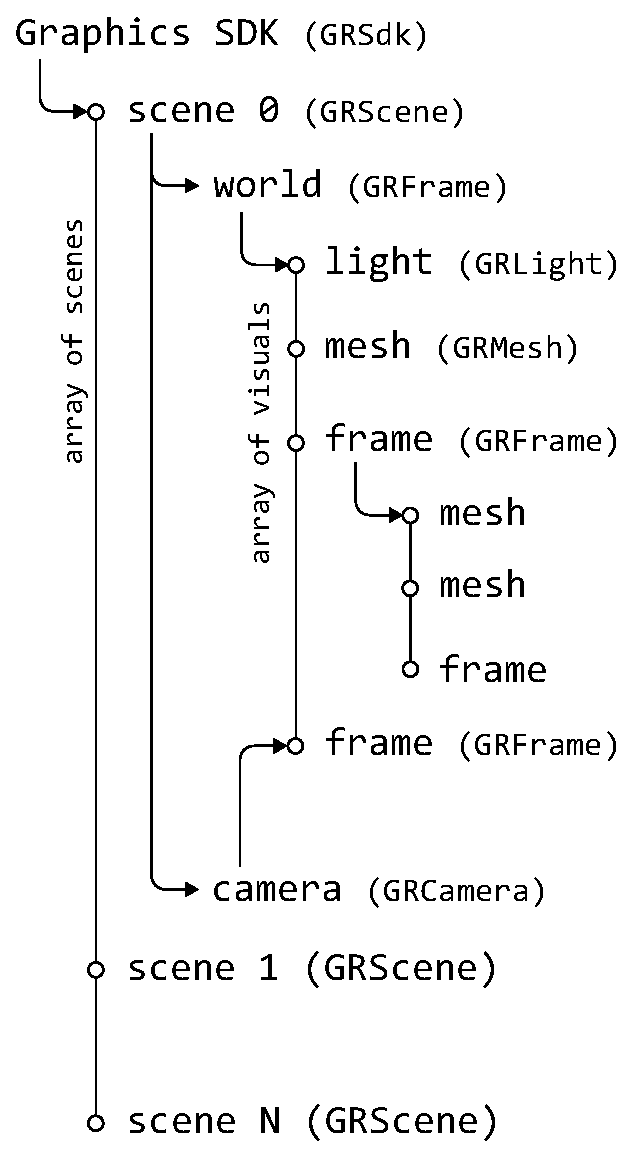
\includegraphics[width=.4\hsize]{fig/grscene.eps}
\end{center}
\caption{Graphics data structure}
\label{fig_grscene}
\end{figure}

\subsection*{シーンの機能}

\KLUDGE シーンを作成したら,次はそのコンテンツであるフレームやメッシュ,カメラやライトなどを作成してシーンに加えていきます.
\KLUDGE この方法としては完全に手動でシーンを構築する他にもFileIOモジュールを使用してファイルからシーンをロードする方法もあります.
\KLUDGE 以下に\texttt{GRScene}の関数を示します.

\begin{center}
\begin{tabular}{p{.15\hsize}p{.45\hsize}p{.3\hsize}}
\texttt{GRSceneIf}	 &															&	\\ \midrule
\texttt{GRFrameIf*}	 & \texttt{GetWorld()}										& ワールドフレームの取得	\\
\texttt{GRCameraIf*} & \texttt{GetCamera()}										& カメラの取得	\\
\texttt{void}		 & \texttt{SetCamera(const GRCameraDesc\&)}					& カメラの設定	\\
\texttt{GRVisualIf*} & \texttt{CreateVisual(const GRVisualDesc\&, GRFrameIf*)}	& 描画アイテムの作成	\\
\texttt{void}		 & \texttt{Render(GRRenderIf*)}								& 描画	\\
\end{tabular}
\end{center}

\KLUDGE %	///	アニメーションコントローラの取得
\KLUDGE %	GRAnimationControllerIf* GetAnimationController();

Fig.\,\ref{fig_grscene}に示すように,1つのシーンはただ1つのワールドフレームを持ち,それを基点として
\KLUDGE 任意の数の描画アイテムがツリー状に連なります.
\KLUDGE ワールドフレームは\texttt{GetWorld}で取得します.

\KLUDGE 特殊な描画アイテムにカメラがあります.
\KLUDGE カメラはワールドフレーム以下のツリーとは別に,\texttt{GRScene}が保持します(Fig.\,\ref{fig_grscene}).
\KLUDGE カメラの設定は\texttt{SetCamera}で行います.
\KLUDGE カメラを取得するには\texttt{GetCamera}を使います.
\KLUDGE また,カメラはシーングラフ中の1つのフレームを参照し,これを視点の設定に用います.
\KLUDGE イメージとしてはカメラが参照先のフレームに取り付けられていると考える方が自然でしょう.
\KLUDGE 参照先のフレームの移動に応じてカメラもシーン中を移動することになります.


\subsection*{シーンの描画}

\KLUDGE 描画処理はプログラムの描画ハンドラで行います.GLUTを使う場合は\texttt{glutDisplayFunc}で登録したコールバック関数がこれにあたり,
\KLUDGE またFrameworkモジュールの\texttt{FWApp}を使う場合は\texttt{Display}仮想関数がこれにあたります.
\KLUDGE 以下が典型的な描画処理です.
\begin{verbatim}
    render->ClearBuffer();        // clear back buffer
    render->BeginScene();         // begin rendering

    grScene->Render(render);      // render scene

    render->EndScene();           // end rendering
    render->SwapBuffers();        // swap buffers
\end{verbatim}

\texttt{ClearBuffer}は描画バッファを所定の色で塗りつぶします.
\KLUDGE 塗りつぶし色の取得/設定は\texttt{GRRender}の\texttt{GetClearColor},\text{SetClearColor}を使います.
\begin{verbatim}
    render->SetClearColor(Vec4f(1.0f, 0.0f, 0.0f, 1.0f));
    render->ClearBuffer();        // clear back buffer in red
\end{verbatim}

\texttt{BeginScene}と\texttt{EndScene}はシーンの描画の前後で必ず呼び出します.
\texttt{SwapBuffers}はフロントバッファとバックバッファを切り換えることで描画内容を画面上に表示します.

\texttt{GRScene}の\texttt{Render}関数は,カメラ(\texttt{GRCamera})の\texttt{Render}とワールドフレーム(\texttt{GRFrame})の\texttt{Render}を
\KLUDGE 順次呼び出します.まずカメラの描画によって視点と投影変換が設定され,
\KLUDGE 次にワールドフレームの描画によってシーングラフが再帰的に描画されます.

\section{描画アイテム}

\begin{figure}[t]
\begin{center}
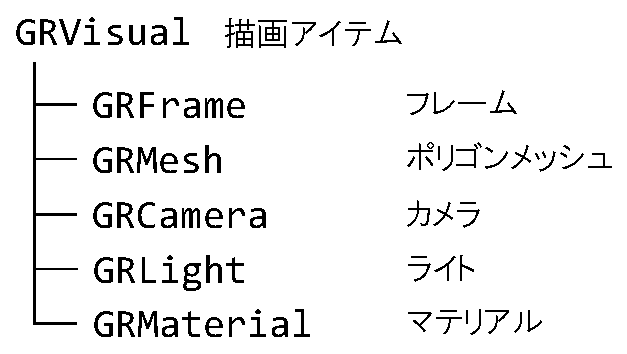
\includegraphics[width=.4\hsize]{fig/grvisual.eps}
\end{center}
\caption{Class hierarchy of visual items}
\label{fig_grvisual}
\end{figure}

\index{GRVisual}
\KLUDGE シーングラフを構成する描画アイテムの基本クラスは\texttt{GRVisual}です.
\texttt{GRVisual}から派生するクラスをFig.\,\ref{fig_grvisual}に示します.
\KLUDGE 描画アイテムには以下の共通の機能があります.

\begin{center}
\begin{tabular}{p{.15\hsize}p{.45\hsize}p{.3\hsize}}
\multicolumn{3}{l}{\texttt{GRVisualIf}}					\\ \midrule
\texttt{void}	& \texttt{Render(GRRenderIf*)}		& 	\\
\texttt{void} 	& \texttt{Rendered(GRRenderIf*)}	& 	\\
\texttt{void} 	& \texttt{Enable(bool)}				& 	\\
\texttt{bool} 	& \texttt{IsEnabled()}				& 	\\
\end{tabular}
\end{center}

\texttt{Render}はアイテムの描画を行い,\texttt{Rendered}は描画の後処理を行います.
\KLUDGE 描画処理は描画アイテムの種類ごとに異なります.
\KLUDGE これについては次節以降で説明します.

\texttt{Enable}関数は描画処理の有効化/無効化を行います.
\KLUDGE 無効化されたアイテムは描画されません.
\texttt{IsEnabled}関数は有効/無効状態を返します.

\KLUDGE 描画アイテムを作成するには\texttt{GRScene}の\texttt{CreateVisual}関数に種類ごとのディスクリプタを指定して呼び出します.


\section{フレーム}

\index{GRFrame}
\index{ふれーむ@フレーム}
\KLUDGE フレームは座標変換を定義すると同時に他の描画アイテムのコンテナとしての役割を持ちます.
\KLUDGE フレームのクラスは\texttt{GRFrame}です.
\KLUDGE 次のコードは,フレームを作成してワールドフレームの子として登録します.
\begin{verbatim}
    GRFrameDesc desc;
    GRFrameIf* frame =
        grScene->CreateVisual(desc, grScene->GetWorldFrame())->Cast();
\end{verbatim}
\texttt{CreateVisual}関数は指定されたディスクリプタに対応する描画アイテムを作成し,
\KLUDGE 指定された親フレームの子として登録します.親フレームを省くとデフォルトでワールドフレームに登録されます.
\KLUDGE したがって上のコードは\texttt{CreateVisual(desc)}としてもかまいません.

\texttt{GRFrame}の\texttt{Render}関数は,子描画アイテムの\texttt{Render}を順次呼び出します.


\subsection*{親子関係}

\KLUDGE フレーム間の親子関係を管理する関数には次のものがあります.

\begin{center}
\begin{tabular}{p{.20\hsize}p{.45\hsize}p{.25\hsize}}
\multicolumn{3}{l}{\texttt{GRFrameIf}}						\\ \midrule
\texttt{GRFrameIf*}		& \texttt{GetParent()}				& 	\\
\texttt{void} 			& \texttt{SetParent(GRFrameIf*)}	& 	\\
\texttt{int} 			& \texttt{NChildren()}				& 	\\
\texttt{GRVisualIf**} 	& \texttt{GetChildren()}			& 	\\
\end{tabular}
\end{center}

\texttt{GetParent}は親フレームを取得します.
\texttt{SetParent}はそのフレームの親フレームを変更するために使います.
\texttt{NChildren}はそのフレームの子である描画アイテムの数を返します.
\KLUDGE これらにはフレーム以外の描画アイテムも含まれることに注意してください.
\texttt{GetChildren}は子描画アイテムの配列を取得します.


\subsection*{座標変換}

\KLUDGE フレームの座標変換を操作する関数は以下の通りです.

\begin{center}
\begin{tabular}{p{.15\hsize}p{.45\hsize}p{.3\hsize}}
\multicolumn{3}{l}{\texttt{GRFrameIf}}							\\ \midrule
\texttt{Affinef} & \texttt{GetTransform()}					& 	\\
\texttt{Affinef} & \texttt{GetWorldTransform()}				& 	\\
\texttt{void}	 & \texttt{SetTransform(const Affinef\&)}	& 	\\
\end{tabular}
\end{center}

\texttt{GetTransform},\texttt{SetTransform}はそれぞれフレームとその親フレームとの間の相対的な座標変換を取得/設定します.
\KLUDGE 例えば
\begin{verbatim}
    frame->SetTransform(Affinef::Trn(1.0, 0.0, 0.0));
\end{verbatim}
\KLUDGE とすると親フレームに対して相対的にx方向に$1.0$移動します.

\section{カメラ}

\begin{figure}[t]
\begin{tabular}{c}
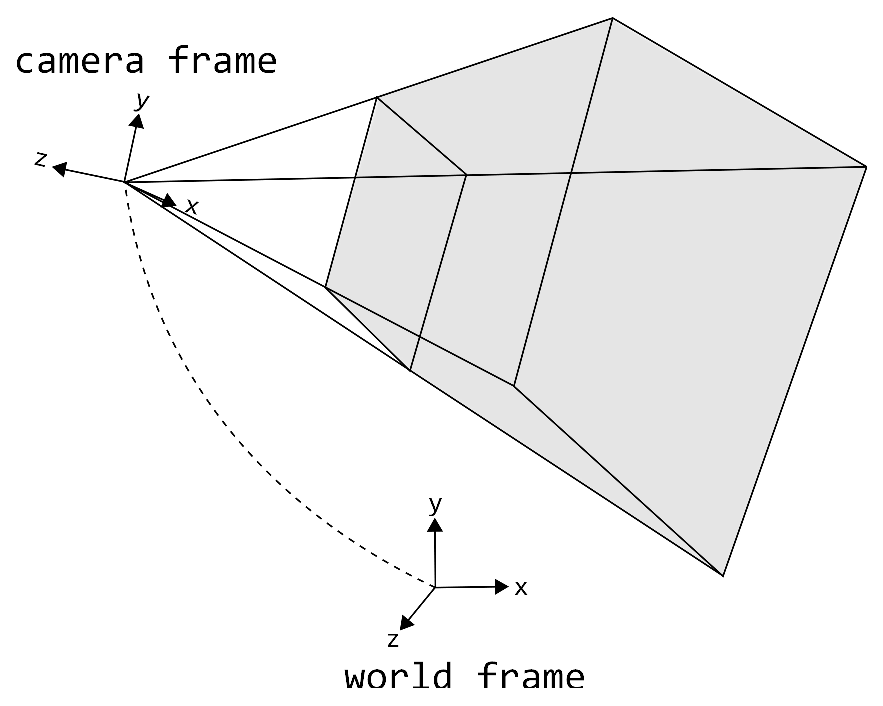
\includegraphics[width=.4\hsize]{fig/grcamera.eps} \\
(a) Perspective frustum \\
\\
\begin{tabular}{cc}
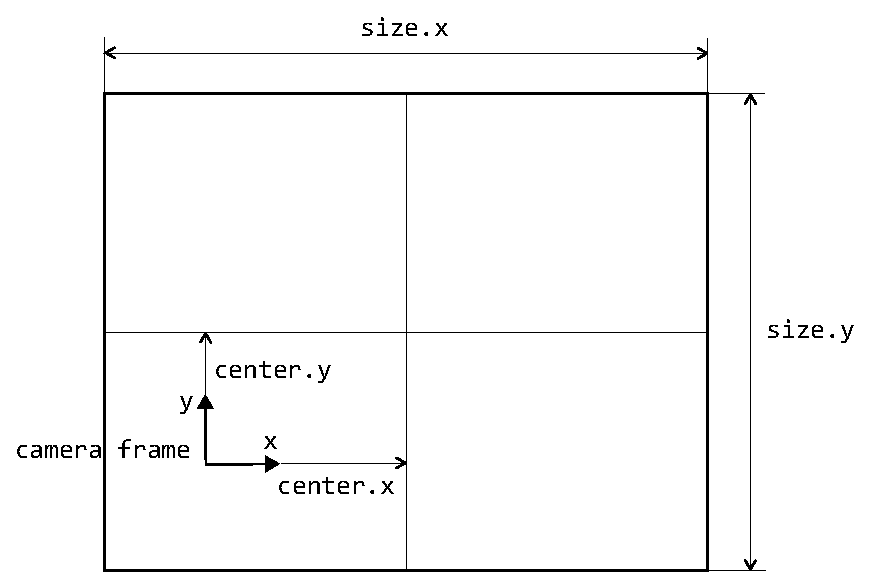
\includegraphics[width=.4\hsize]{fig/grcamera_front.eps} &
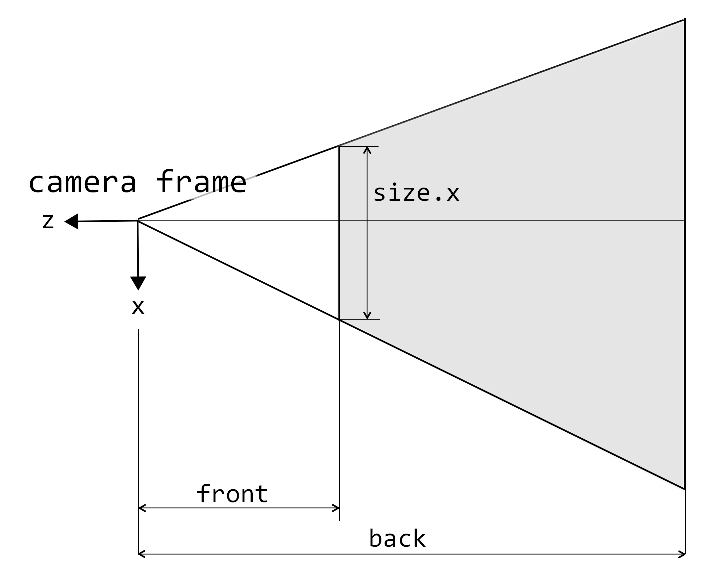
\includegraphics[width=.4\hsize]{fig/grcamera_top.eps} \\
(b) Front view of screen &
(c) Top view of screen
\end{tabular}
\end{tabular}
\caption{Camera parameters}
\label{fig_grcamera}
\end{figure}

\index{GRCamera}
\index{かめら@カメラ}
\KLUDGE カメラは描画における視点の設定と投影変換を管理します.
\KLUDGE はじめにカメラのディスクリプタを見ていきます.

\begin{center}
\begin{tabular}{p{.15\hsize}p{.45\hsize}p{.3\hsize}}
\multicolumn{3}{l}{\texttt{GRCameraDesc}}					\\ \midrule
\texttt{Vec2f}	&	\texttt{size}	& スクリーンサイズ 		\\
\texttt{Vec2f}	&	\texttt{center}	& スクリーン中心座標 	\\
\texttt{float}	&	\texttt{front}	& 前方クリップ面		\\
\texttt{float}	&	\texttt{back}	& 後方クリップ面		\\
\end{tabular}
\end{center}

\KLUDGE 各変数の定義はFig.\,\ref{fig_grcamera}(b),(c)を参照してください.
\KLUDGE 設定を変更するには以下のようにします.
\begin{verbatim}
    GRCameraDesc desc;
    grScene->GetCamera()->GetDesc(&desc);
    desc.front = 3.0f;
    grScene->SetCamera(desc);
\end{verbatim}
\KLUDGE 上では\texttt{GetDesc}関数で既存の設定をディスクリプタにコピーし,\texttt{front}を変更してから
\texttt{SetCamera}関数で再設定しています.

\KLUDGE 一方,\texttt{GRCamera}の関数は以下の通りです.

\begin{center}
\begin{tabular}{p{.15\hsize}p{.45\hsize}p{.3\hsize}}
\multicolumn{3}{l}{\texttt{GRCameraIf}}					\\ \midrule
\texttt{GRFrameIf*}	& \texttt{GetFrame()}				&	\\
\texttt{void}		& \texttt{SetFrame(GRFrameIf*)}		&	\\
\end{tabular}
\end{center}

\texttt{GetFrame},\texttt{SetFrame}関数はカメラフレームを取得/設定します.
Fig.\,\ref{fig_grcamera}(a)のように,カメラフレームはカメラの視点を定義します.

\section{ライト}

\index{GRLight}
\index{らいと@ライト}
\KLUDGE ライトはシーンの照明を設定するための描画アイテムです.
\KLUDGE ライトのクラス\texttt{GRLight}のディスクリプタの代表的な変数を以下に示します.

\begin{center}
\begin{tabular}{p{.15\hsize}p{.45\hsize}p{.3\hsize}}
\multicolumn{3}{l}{\texttt{GRLightDesc}}				\\ \midrule
\texttt{Vec4f}	&	\texttt{ambient}	& 環境光 		\\
\texttt{Vec4f}	&	\texttt{diffuse}	& 拡散光 		\\
\texttt{Vec4f}	&	\texttt{specular}	& 鏡面光		\\
\texttt{Vec4f}	&	\texttt{position}	& ライト位置	\\
\end{tabular}
\end{center}

\KLUDGE 減衰係数やスポットライトなどのより詳細な設定項目についてはソースファイルを参照してください.
OpenGLの仕様と同様,\texttt{position}の第4成分\texttt{position.w}が$0$の場合は平行光源となり,
\texttt{(x,y,z)}方向の無限遠にライトがあることになり,\texttt{position.w}が$1$の場合は
\texttt{(x,y,z)}の位置に点光源がおかれます.

\section{マテリアル}
\label{sec_grmaterial}

\index{GRMaterial}
\index{まてりある@マテリアル}
\KLUDGE マテリアルは材質を指定するためのアイテムです.
\KLUDGE マテリアルのクラスは\texttt{GRMaterial}です.
\KLUDGE 通常,マテリアルは次節で説明するメッシュの子描画アイテムとなります.
\KLUDGE ファイルからメッシュをロードする場合は,メッシュの作成と同時にマテリアルも自動的に作成され,メッシュの子として追加されます.
\texttt{GRMaterial}のディスクリプタは以下の通りです.

\begin{center}
\begin{tabular}{p{.15\hsize}p{.45\hsize}p{.3\hsize}}
\multicolumn{3}{l}{\texttt{GRMaterialDesc}}				\\ \midrule
\texttt{Vec4f}		&	\texttt{ambient}	& 環境色 	\\
\texttt{Vec4f}		&	\texttt{diffuse}	& 拡散色 	\\
\texttt{Vec4f}		&	\texttt{specular}	& 鏡面色	\\
\texttt{Vec4f}		&	\texttt{emissive}	& 自己発光	\\
\texttt{float}		&	\texttt{power}		& 鏡面係数	\\
\texttt{UTString}	&	\texttt{texname}	& テクスチャファイル名
\end{tabular}
\end{center}

\KLUDGE レンダラにマテリアルを設定すると,次に別のマテリアルを設定するまでの間の
\KLUDGE 形状描画にそのマテリアルの描画属性が適用されます.
\KLUDGE マテリアルを設定するにはいくつかの方法があります.
\KLUDGE 一つ目は\texttt{GRMaterialIf}の\texttt{Render}関数を呼ぶ方法です:
\KLUDGE これに加え,以下に示す\texttt{GRRender}の関数のいずれかを用いることもできます.
\begin{center}
\begin{tabular}{p{.1\hsize}p{.5\hsize}p{.3\hsize}}
\texttt{GRRenderIf}																\\ \midrule
\texttt{void} & \texttt{SetMaterial(const GRMaterialDesc\&)}		& 描画マテリアルの設定	\\
\texttt{void} & \texttt{SetMaterial(const GRMaterialIf*)}			& 描画マテリアルの設定	\\
\texttt{void} & \texttt{SetMaterial(int)}							& 描画マテリアルの設定	\\
\end{tabular}
\end{center}
\KLUDGE 以下の例はマテリアルを設定する3通りの方法を示しています.
\KLUDGE どの方法を用いても結果は変わりません.
\begin{verbatim}
    // given GRRenderIf* render, GRSceneIf* scene
    GRMaterialDesc md;
    md.diffuse = Vec4f(1.0f, 0.0f, 0.0f, 1.0f);
    // 1.
    render->SetMaterial(md);
    // 2.
    GRMaterialIf* mat = scene->CreateVisual(md)->Cast();
    mat->Render(render);
    // 3.
    render->SetMaterial(mat);
\end{verbatim}
\KLUDGE 毎回マテリアルを作成するのは煩わしいことがあります.
\KLUDGE そのような場合はレンダラの予約色を指定することも可能です.
\begin{verbatim}
    // 4.
    render->SetMaterial(GRRenderBaseIf::RED);
\end{verbatim}
\KLUDGE 使用可能な予約色はX11 web colorにもとづいています.
\KLUDGE 詳しくは\texttt{SprGRRender.h}ヘッダファイルを

\KLUDGE %%%%%%%%%%%%%%%%%%%%%%%%%%%%%%%%%%%%%%%%%%%%%%%%%%%%%%%%%%%%%%%%%%%%%%%%%%%%%%%%%%%%%%
\begin{comment}

\begin{table}[t]
\caption{Reserved colors}
\label{table_material_sample}
{\small
\begin{center}
\begin{tabular}{ll|ll}
RED				& {\color[RGB]{255,0,0}$\blacksquare$} 			(1.00, 0.00, 0.00)	&
GREEN			& {\color[rgb]{0,1,0}$\blacksquare$} 			(0.00, 1.00, 0.00)	\\
BLUE			& {\color[rgb]{0,0,1}$\blacksquare$} 			(0.00, 0.00, 1.00)	&
YELLOW			& {\color[rgb]{1,1,0}$\blacksquare$} 			(1.00, 1.00, 0.00)	\\
CYAN			& {\color[rgb]{0,1,1}$\blacksquare$} 			(0.00, 1.00, 1.00)	&
MAGENTA			& {\color[rgb]{1,0,1}$\blacksquare$} 			(1.00, 0.00, 1.00)	\\
WHITE			& {$\square$} 						 			(1.00, 1.00, 1.00)	&
GRAY			& {\color[rgb]{.5,.5,.5}$\blacksquare$} 		(0.50, 0.50, 0.50)	\\
ORANGE			& {\color[rgb]{1,.27,0}$\blacksquare$} 			(1.00, 0.27, 0.00)	&
BROWN			& {\color[rgb]{.198,0,0}$\blacksquare$} 		(0.19, 0.00, 0.00)	\\
LIGHT\_BLUE		& {\color[rgb]{.676,.844,.898}$\blacksquare$} 	(0.67, 0.84, 0.89)	&
MEDIUM\_PURPLE	& {\color[rgb]{.574,.438,.855}$\blacksquare$} 	(0.57, 0.43, 0.85)	\\
DARK\_GREEN		& {\color[rgb]{0,.391,0}$\blacksquare$} 		(0.00, 0.39, 0.00)	&
DARK\_VIOLET	& {\color[rgb]{.578,0,.824}$\blacksquare$} 		(0.57, 0.00, 0.82)	\\
DARK\_CYAN		& {\color[rgb]{0,.543,.543}$\blacksquare$} 		(0.00, 0.54, 0.54)	&
GREEN\_YELLOW	& {\color[rgb]{.676,1,.184}$\blacksquare$} 		(0.67, 1.00, 0.18)	\\
LIME\_GREEN		& {\color[rgb]{.195,.801,.195}$\blacksquare$} 	(0.19, 0.80, 0.19)	&
INDIAN\_RED		& {\color[rgb]{.801,.359,.359}$\blacksquare$} 	(0.80, 0.35, 0.35)	\\
INDIGO			& {\color[rgb]{.293,0,.508}$\blacksquare$} 		(0.29, 0.00, 0.50)	&
GREEN\_INDIGO	& {\color[rgb]{0,.198,.198}$\blacksquare$} 		(0.00, 0.19, 0.19)	\\
OLIVE\_GREEN	& {\color[rgb]{.198,.398,0}$\blacksquare$} 		(0.19, 0.39, 0.00)	&
NAVY\_BLUE		& {\color[rgb]{.198,.398,.797}$\blacksquare$} 	(0.19, 0.39, 0.79)	\\
TURQUOISE\_BLUE	& {\color[rgb]{.398,1,.797}$\blacksquare$} 		(0.39, 1.00, 0.79)	&
EMERALD\_GREEN	& {\color[rgb]{.598,1,.398}$\blacksquare$} 		(0.59, 1.00, 0.39)
\end{tabular}
\end{center}
}
\end{table}

\end{comment}
\KLUDGE %%%%%%%%%%%%%%%%%%%%%%%%%%%%%%%%%%%%%%%%%%%%%%%%%%%%%%%%%%%%%%%%%%%%%%%%%%%%%%%%%%%%%%

\begin{table}[t]
\caption{Reserved colors}
\label{table_material_sample}
{\tiny
\begin{center}
\ifLwarp\else
\begin{tabular}{l|l}
\fi
\begin{tabular}{lll}
INDIANRED		& {\color[RGB]{205,92,92}$\blacksquare$}	& (205 92 92) \\
LIGHTCORAL		& {\color[RGB]{240,128,128}$\blacksquare$}	& (240 128 128) \\
SALMON			& {\color[RGB]{250,128,114}$\blacksquare$}	& (250 128 114) \\
DARKSALMON		& {\color[RGB]{233,150,122}$\blacksquare$}	& (233 150 122) \\
LIGHTSALMON		& {\color[RGB]{255,160,122}$\blacksquare$}	& (255 160 122) \\
RED				& {\color[RGB]{255,0,0}$\blacksquare$}		& (255 0 0) \\
CRIMSON			& {\color[RGB]{220,20,60}$\blacksquare$}	& (220 20 60) \\
FIREBRICK		& {\color[RGB]{178,34,34}$\blacksquare$}	& (178 34 34) \\
DARKRED			& {\color[RGB]{139,0,0}$\blacksquare$}		& (139 0 0) \\
\\
PINK			& {\color[RGB]{255,192,203}$\blacksquare$}	& (255 192 203)	\\
LIGHTPINK		& {\color[RGB]{255,182,193}$\blacksquare$}	& (255 182 193)	\\
HOTPINK			& {\color[RGB]{255,105,180}$\blacksquare$}	& (255 105 180)	\\
DEEPPINK		& {\color[RGB]{255, 20,147}$\blacksquare$}	& (255  20 147)	\\
MEDIUMVIOLETRED	& {\color[RGB]{199, 21,133}$\blacksquare$}	& (255  21 133)	\\
PALEVIOLETRED	& {\color[RGB]{219,112,147}$\blacksquare$}	& (255 112 147)	\\
\\
CORAL			& {\color[RGB]{255,127, 80}$\blacksquare$}	& (255 127 80)	\\
TOMATO			& {\color[RGB]{255, 99, 71}$\blacksquare$}	& (255  99 71)	\\
ORANGERED		& {\color[RGB]{255, 69,  0}$\blacksquare$}	& (255  69 0)	\\
DARKORANGE		& {\color[RGB]{255,140,  0}$\blacksquare$}	& (255 140 0)	\\
ORANGE			& {\color[RGB]{255,165,  0}$\blacksquare$}	& (255 165 0)	\\
\\
GOLD					& {\color[RGB]{255,215,0}$\blacksquare$}	& (255 215 0)	\\
YELLOW					& {\color[RGB]{255,255,0}$\blacksquare$}	& (255 255 0)	\\
LIGHTYELLOW				& {\color[RGB]{255,255,224}$\blacksquare$}	& (255 255 224)	\\
LEMONCHIFFON			& {\color[RGB]{255,250,205}$\blacksquare$}	& (255 250 205)	\\
LIGHTGOLDENRODYELLOW	& {\color[RGB]{250,250,210}$\blacksquare$}	& (250 250 210)	\\
PAPAYAWHIP				& {\color[RGB]{255,239,213}$\blacksquare$}	& (255 239 213)	\\
MOCCASIN				& {\color[RGB]{255,228,181}$\blacksquare$}	& (255 228 181)	\\
PEACHPUFF				& {\color[RGB]{255,218,185}$\blacksquare$}	& (255 218 185)	\\
PALEGOLDENROD			& {\color[RGB]{238,232,170}$\blacksquare$}	& (238 232 170)	\\
KHAKI					& {\color[RGB]{240,230,140}$\blacksquare$}	& (240 230 140)	\\
DARKKHAKI				& {\color[RGB]{189,183,107}$\blacksquare$}	& (189 183 107)	\\
\\						
LAVENDAR				& {\color[RGB]{230,230,250}$\blacksquare$}	& (230 230 250)	\\
THISTLE					& {\color[RGB]{216,191,216}$\blacksquare$}	& (216 191 216)	\\
PLUM					& {\color[RGB]{221,160,221}$\blacksquare$}	& (221 160 221)	\\
VIOLET					& {\color[RGB]{238,130,238}$\blacksquare$}	& (238 130 238)	\\
ORCHILD					& {\color[RGB]{218,112,214}$\blacksquare$}	& (218 112 214)	\\
FUCHSIA					& {\color[RGB]{255,0,255}$\blacksquare$}	& (255 0 255)	\\
MAGENTA					& {\color[RGB]{255,0,255}$\blacksquare$}	& (255 0 255)	\\
MEDIUMORCHILD			& {\color[RGB]{186,85,211}$\blacksquare$}	& (186 85 211)	\\
MEDIUMPURPLE			& {\color[RGB]{147,112,219}$\blacksquare$}	& (147 112 219)	\\
BLUEVIOLET				& {\color[RGB]{138,43,226}$\blacksquare$}	& (138 43 226)	\\
DARKVIOLET				& {\color[RGB]{148,0,211}$\blacksquare$}	& (148 0 211)	\\
DARKORCHILD				& {\color[RGB]{153,50,204}$\blacksquare$}	& (153 50 204)	\\
DARKMAGENTA				& {\color[RGB]{139,0,139}$\blacksquare$}	& (139 0 139)	\\
PURPLE					& {\color[RGB]{128,0,128}$\blacksquare$}	& (128 0 128)	\\
INDIGO					& {\color[RGB]{75,0,130}$\blacksquare$}	& (75 0 130)	\\
DARKSLATEBLUE			& {\color[RGB]{72,61,139}$\blacksquare$}	& (72 61 139)	\\
SLATEBLUE				& {\color[RGB]{106,90,205}$\blacksquare$}	& (106 90 205)	\\
MEDIUMSLATEBLUE			& {\color[RGB]{123,104,238}$\blacksquare$}	& (123 104 238)	\\
\\
GREENYELLOW				& {\color[RGB]{173,255,47}$\blacksquare$}	& (173 255 47)	\\
CHARTREUSE				& {\color[RGB]{127,255,0}$\blacksquare$}	& (127 255 0)	\\
LAWNGREEN				& {\color[RGB]{124,252,0}$\blacksquare$}	& (124 252 0)	\\
LIME					& {\color[RGB]{0,255,0}$\blacksquare$}	& (0 255 0)	\\
LIMEGREEN				& {\color[RGB]{50,205,50}$\blacksquare$}	& (50 205 50)	\\
PALEGREEN				& {\color[RGB]{152,251,152}$\blacksquare$}	& (152 251 152)	\\
LIGHTGREEN				& {\color[RGB]{144,238,144}$\blacksquare$}	& (144 238 144)	\\
MEDIUMSPRINGGREEN		& {\color[RGB]{0,250,154}$\blacksquare$}	& (0 250 154)	\\
SPRINGGREEN				& {\color[RGB]{0,255,127}$\blacksquare$}	& (0 255 127)	\\
MEDIUMSEAGREEN			& {\color[RGB]{60,179,113}$\blacksquare$}	& (60 179 113)	\\
SEAGREEN				& {\color[RGB]{46,139,87}$\blacksquare$}	& (46 139 87)	\\
FORESTGREEN				& {\color[RGB]{34,139,34}$\blacksquare$}	& (34 139 34)	\\
GREEN					& {\color[RGB]{0,128,0}$\blacksquare$}	& (0 128 0)	\\
DARKGREEN				& {\color[RGB]{0,100,0}$\blacksquare$}	& (0 100 0)	\\
YELLOWGREEN				& {\color[RGB]{154,205,50}$\blacksquare$}	& (154 205 50)	\\
OLIVEDRAB				& {\color[RGB]{107,142,35}$\blacksquare$}	& (107 142 35)	\\
OLIVE					& {\color[RGB]{128,128,0}$\blacksquare$}	& (128 128 0)	\\
DARKOLIVEGREEN			& {\color[RGB]{85,107,47}$\blacksquare$}	& (85 107 47)	\\
MEDIUMAQUAMARINE		& {\color[RGB]{102,205,170}$\blacksquare$}	& (102 205 170)	\\
DARKSEAGREEN			& {\color[RGB]{143,188,143}$\blacksquare$}	& (143 188 143)	\\
LIGHTSEAGREEN			& {\color[RGB]{32,178,170}$\blacksquare$}	& (32 178 170)	\\
DARKCYAN				& {\color[RGB]{0,139,139}$\blacksquare$}	& (0 139 139)	\\
TEAL					& {\color[RGB]{0,128,128}$\blacksquare$}	& (0 128 128)	\\
\\
\end{tabular}
\ifLwarp\vspace{2\baselineskip}\else
&
\fi
\begin{tabular}{lll}
AQUA				& {\color[RGB]{0,255,255}$\blacksquare$}	& (0 255 255)	\\
CYAN				& {\color[RGB]{0,255,255}$\blacksquare$}	& (0 255 255)	\\
LIGHTCYAN			& {\color[RGB]{224,255,255}$\blacksquare$}	& (224 255 255)	\\
PALETURQUOISE		& {\color[RGB]{175,238,238}$\blacksquare$}	& (175 238 238)	\\
AQUAMARINE			& {\color[RGB]{127,255,212}$\blacksquare$}	& (127 255 212)	\\
TURQUOISE			& {\color[RGB]{64,224,208}$\blacksquare$}	& (64 224 208)	\\
MEDIUMTURQUOISE		& {\color[RGB]{72,209,204}$\blacksquare$}	& (72 209 204)	\\
DARKTURQUOISE		& {\color[RGB]{0,206,209}$\blacksquare$}	& (0 206 209)	\\
CADETBLUE			& {\color[RGB]{95,158,160}$\blacksquare$}	& (95 158 160)	\\
STEELBLUE			& {\color[RGB]{70,130,180}$\blacksquare$}	& (70 130 180)	\\
LIGHTSTEELBLUE		& {\color[RGB]{176,196,222}$\blacksquare$}	& (176 196 222)	\\
POWDERBLUE			& {\color[RGB]{176,224,230}$\blacksquare$}	& (176 224 230)	\\
LIGHTBLUE			& {\color[RGB]{173,216,230}$\blacksquare$}	& (173 216 230)	\\
SKYBLUE				& {\color[RGB]{135,206,235}$\blacksquare$}	& (135 206 235)	\\
LIGHTSKYBLUE		& {\color[RGB]{135,206,250}$\blacksquare$}	& (135 206 250)	\\
DEEPSKYBLUE			& {\color[RGB]{0,191,255}$\blacksquare$}	& (0 191 255)	\\
DODGERBLUE			& {\color[RGB]{30,144,255}$\blacksquare$}	& (30 144 237)	\\
CORNFLOWERBLUE		& {\color[RGB]{100,149,237}$\blacksquare$}	& (65 105 225)	\\
ROYALBLUE			& {\color[RGB]{65,105,225}$\blacksquare$}	& (65 105 225)	\\
BLUE				& {\color[RGB]{0,0,255}$\blacksquare$}	& (0 0 255)	\\
MEDIUMBLUE			& {\color[RGB]{0,0,205}$\blacksquare$}	& (0 0 205)	\\
DARKBLUE			& {\color[RGB]{0,0,139}$\blacksquare$}	& (0 0 139)	\\
NAVY				& {\color[RGB]{0,0,128}$\blacksquare$}	& (0 0 128)	\\
MIDNIGHTBLUE		& {\color[RGB]{25,25,112}$\blacksquare$}	& (25 25 112)	\\
\\
CORNSILK			& {\color[RGB]{255,248,220}$\blacksquare$}	& (255 248 220)	\\
BLANCHEDALMOND		& {\color[RGB]{255,235,205}$\blacksquare$}	& (255 235 205)	\\
BISQUE				& {\color[RGB]{255,228,196}$\blacksquare$}	& (255 228 196)	\\
NAVAJOWHITE			& {\color[RGB]{255,222,173}$\blacksquare$}	& (255 222 173)	\\
WHEAT				& {\color[RGB]{245,222,179}$\blacksquare$}	& (245 222 179)	\\
BURLYWOOD			& {\color[RGB]{222,184,135}$\blacksquare$}	& (222 184 135)	\\
TAN					& {\color[RGB]{210,180,140}$\blacksquare$}	& (210 180 140)	\\
ROSYBROWN			& {\color[RGB]{188,143,143}$\blacksquare$}	& (188 143 143)	\\
SANDYBROWN			& {\color[RGB]{244,164,96}$\blacksquare$}	& (244 164 96)	\\
GOLDENROD			& {\color[RGB]{218,165,32}$\blacksquare$}	& (218 165 32)	\\
DARKGOLDENROD		& {\color[RGB]{184,134,11}$\blacksquare$}	& (184 134 11)	\\
PERU				& {\color[RGB]{205,133,63}$\blacksquare$}	& (205 133 63)	\\
CHOCOLATE			& {\color[RGB]{210,105,30}$\blacksquare$}	& (210 105 30)	\\
SADDLEBROWN			& {\color[RGB]{139,69,19}$\blacksquare$}	& (139 69 19)	\\
SIENNA				& {\color[RGB]{160,82,45}$\blacksquare$}	& (160 82 45)	\\
BROWN				& {\color[RGB]{154,42,42}$\blacksquare$}	& (154 42 42)	\\
MAROON				& {\color[RGB]{128,0,0}$\blacksquare$}	& (128 0 0)	\\
\\
WHITE				& {\color[RGB]{255,255,255}$\blacksquare$}	& (255 255 255)	\\
SNOW				& {\color[RGB]{255,250,250}$\blacksquare$}	& (255 250 250)	\\
HONEYDEW			& {\color[RGB]{240,255,240}$\blacksquare$}	& (240 255 240)	\\
MINTCREAM			& {\color[RGB]{245,255,250}$\blacksquare$}	& (245 255 250)	\\
AZURE				& {\color[RGB]{240,255,255}$\blacksquare$}	& (240 255 255)	\\
ALICEBLUE			& {\color[RGB]{240,248,255}$\blacksquare$}	& (240 248 255)	\\
GHOSTWHITE			& {\color[RGB]{248,248,255}$\blacksquare$}	& (248 248 255)	\\
WHITESMOKE			& {\color[RGB]{245,245,245}$\blacksquare$}	& (245 245 245)	\\
SEASHELL			& {\color[RGB]{255,245,238}$\blacksquare$}	& (255 245 238)	\\
BEIGE				& {\color[RGB]{245,245,220}$\blacksquare$}	& (245 245 220)	\\
OLDLACE				& {\color[RGB]{253,245,230}$\blacksquare$}	& (253 245 230)	\\
FLORALWHITE			& {\color[RGB]{255,250,240}$\blacksquare$}	& (255 250 240)	\\
IVORY				& {\color[RGB]{255,255,240}$\blacksquare$}	& (255 255 240)	\\
ANTIQUEWHITE		& {\color[RGB]{250,235,215}$\blacksquare$}	& (250 235 215)	\\
LINEN				& {\color[RGB]{250,240,230}$\blacksquare$}	& (250 240 230)	\\
LAVENDERBLUSH		& {\color[RGB]{255,240,245}$\blacksquare$}	& (255 240 245)	\\
MISTYROSE			& {\color[RGB]{255,228,225}$\blacksquare$}	& (255 228 225)	\\
\\
GAINSBORO			& {\color[RGB]{220,220,220}$\blacksquare$}	& (220 220 220)	\\
LIGHTGRAY			& {\color[RGB]{211,211,211}$\blacksquare$}	& (211 211 211)	\\
SILVER				& {\color[RGB]{192,192,192}$\blacksquare$}	& (192 192 192)	\\
DARKGRAY			& {\color[RGB]{169,169,169}$\blacksquare$}	& (169 169 169)	\\
GRAY				& {\color[RGB]{128,128,128}$\blacksquare$}	& (128 128 128)	\\
DIMGRAY				& {\color[RGB]{105,105,105}$\blacksquare$}	& (105 105 105)	\\
LIGHTSLATEGRAY		& {\color[RGB]{119,136,153}$\blacksquare$}	& (119 136 153)	\\
SLATEGRAY			& {\color[RGB]{112,128,144}$\blacksquare$}	& (112 128 144)	\\
DARKSLATEGRAY		& {\color[RGB]{47,79,79}$\blacksquare$}	& (47 79 79)	\\
BLACK				& {\color[RGB]{0,0,0}$\blacksquare$}	& (0 0 0)	\\
\\
\\
\\
\\
\\
\\
\\
\end{tabular}
\ifLwarp\else
\end{tabular}
\fi
\end{center}
}
\end{table}

\texttt{GRRenderBaseIf}が持つ予約色(全24色,Table\,\ref{table_material_sample}参照)です.

\section{メッシュ}

\index{GRMesh}
\index{めっしゅ@メッシュ}
\KLUDGE メッシュは多面体形状を表現するための描画アイテムです.
\KLUDGE メッシュのクラスは\texttt{GRMesh}です.
\KLUDGE メッシュを作成する方法には
\begin{itemize}
\item ディスクリプタを用いて手動で作成する
\item FileIOモジュールを利用してファイルからメッシュをロードする
\end{itemize}
\KLUDGE の二通りがあります.
\KLUDGE 後者の方法では,モデリングソフトで作成し,Direct3DのX形式などで出力したファイルから形状をロードすることができます.
\KLUDGE 詳しくは\ref{chap_fileio}章を参照してください.
\KLUDGE また,メッシュのみをロードする簡易機能として\texttt{FWObjectIf::LoadMesh}が用意されています.

\KLUDGE 以下では前者の手動構築の方法について説明します.
\KLUDGE メッシュのディスクリプタは次の通りです.
\begin{center}
\begin{tabular}{p{.3\hsize}p{.3\hsize}p{.3\hsize}}
\multicolumn{3}{l}{\texttt{GRMeshDesc}}					\\ \midrule
\texttt{vector<Vec3f>}		&	\texttt{vertices}		& 頂点	 			\\
\texttt{vector<GRMeshFace>}	&	\texttt{faces}			& 面	 			\\
\texttt{vector<Vec3f>}		&	\texttt{normals}		& 法線				\\
\texttt{vector<GRMeshFace>}	&	\texttt{faceNormals}	& 面法線			\\
\texttt{vector<Vec4f>}		&	\texttt{colors}			& 色				\\
\texttt{vector<Vec2f>}		&	\texttt{texCoords}		& テクスチャ座標	\\
\texttt{vector<int>}		&	\texttt{materialList}	& マテリアルリスト
\end{tabular}
\end{center}
\texttt{vector}は\texttt{C++}の可変長配列コンテナです.
\texttt{vertices}は頂点座標を格納した配列です.
\KLUDGE ただし頂点座標を設定しただけでは形状は定義されません.
\KLUDGE メッシュは面の集合ですので,\texttt{faces}を設定する必要があります.
\texttt{GRMeshFace}の定義は以下の通りです.
\begin{center}
\begin{tabular}{p{.3\hsize}p{.3\hsize}p{.3\hsize}}
\multicolumn{3}{l}{\texttt{GRMeshFace}}					\\ \midrule
\texttt{int}	&	\texttt{nVertices}		& 頂点数 	\\
\texttt{int}	&	\texttt{indices[4]}		& 頂点インデックス
\end{tabular}
\end{center}
\texttt{nVertices}は1つの面を構成する頂点数で,3か4を設定します.
\texttt{indices}には\texttt{nVertices}個の頂点インデックスを設定します.
\KLUDGE このとき
\begin{align*}
\texttt{vertices[faces[i].indices[j]]}
\end{align*}
\KLUDGE が$i$番目の面の$j$番目の頂点座標となります.

\texttt{GRMeshDesc}のメンバ変数の中で\texttt{vertices}と\texttt{faces}は必須ですが,
\KLUDGE その他のメンバは必ずしも設定する必要はありません.
\texttt{normals}は各頂点の法線の向きをを格納する配列です.
\texttt{normals[i]}が\texttt{vertices[i]}の法線を与えます.
\texttt{normals}を省略した場合,法線は自動生成されます.
\KLUDGE このとき,各頂点の法線はその頂点を共有する面の法線の平均で与えられます.

\texttt{normals}に加えて\texttt{faceNormals}を設定した場合,異なる方法で法線が与えられます.
\KLUDGE このとき
\begin{align*}
\texttt{normals[faceNormals[i].indices[j]]}
\end{align*}
\KLUDGE が$i$番目の面の$j$番目の頂点に対応する法線となります.

\texttt{colors}は頂点色です.\texttt{colors[i]}が$i$番目の頂点の色を与えます.

\texttt{texCoords}は頂点ごとのテクスチャUV座標を与えます.
\KLUDGE テクスチャを描画するには,メッシュに割り当てるマテリアルにテクスチャファイル名が設定されている必要があります.

\texttt{materialList}は面ごとに異なるマテリアルを割り当てるために用います.
\texttt{materialList[i]}が$i$番目の面のマテリアル番号を与えます.
\KLUDGE ただし,番号に対応するマテリアルは別途メッシュに割り当てておく必要があります.

\subsection*{メッシュへのマテリアルの割当て}

\KLUDGE ファイルからメッシュをロードする場合,もしファイル中にマテリアル情報が含まれていれば
\KLUDGE それをもとに自動的にマテリアルがメッシュへ割り当てられます.

\KLUDGE 手動でメッシュに割り当てるには,\texttt{AddChildObject}を使います.
\KLUDGE 以下に例を示します.
\begin{verbatim}
    // given GRSceneIf* scene, GRFrameIf* frame
    GRMeshDesc meshDesc;
    // ... setup discriptor here ...

    // create mesh and attach it to frame
    GRMeshIf* mesh = scene->CreateVisual(meshDesc, frame)->Cast();

    GRMaterialDesc matDesc0, matDesc1;
    // ... setup materials here ...
    GRMaterialIf* mat0 = scene->CreateVisual(matDesc0, frame)->Cast();
    GRMaterialIf* mat1 = scene->CreateVisual(matDesc1, frame)->Cast();

    // attach materials to mesh
    mesh->AddChildObject(mat0);    //< material no.0
    mesh->AddChildObject(mat1);    //< material no.1
\end{verbatim}
\KLUDGE 最初に割り当てられたマテリアルを0番として昇順でマテリアル番号が決まります.
\KLUDGE 前述のマテリアルリストを用いる場合はこのマテリアル番号を面毎に指定してください.


\section{レンダラ}

\index{GRRender}
\index{レンダラ}
\KLUDGE レンダラの機能を項目別に説明します.
\KLUDGE レンダラは提供するプリミティブな描画機能は非常に多岐に渡りますが,これらのほとんどの関数は特別な描画処理を必要としない限りユーザが直接呼び出すことはありません.
\KLUDGE 個々の関数を詳しく説明していくと膨大な量になりますので,ここでは一覧程度にとどめます.
\KLUDGE 詳細な仕様はソースコードのコメントを参照してください.

\subsection*{基本機能}

\KLUDGE 描画時のお決まりの処理です.
\ref{sec_grscene}節を参照してください.

\begin{center}
\begin{tabular}{p{.1\hsize}p{.45\hsize}p{.35\hsize}}
\multicolumn{2}{l}{\texttt{GRRenderIf}}									\\ \midrule
\texttt{void} & \texttt{GetClearColor(Vec4f\&)}			& 背景色の取得				\\
\texttt{void} & \texttt{SetClearColor(const Vec4f\&)}	& 背景色の設定				\\
\texttt{void} & \texttt{ClearBuffer()}					& 描画バッファをクリア		\\
\texttt{void} & \texttt{BeginScene()}					& 描画の開始				\\
\texttt{void} & \texttt{EndScene()}						& 描画の完了				\\
\texttt{void} & \texttt{SwapBuffers()}					& 描画バッファのスワップ	\\
\end{tabular}
\end{center}

\subsection*{ディスプレイリスト}

\KLUDGE ディスプレイリストに関係する機能です.
\texttt{GRMesh}が内部で使用します.

\begin{center}
\begin{tabular}{p{.1\hsize}p{.45\hsize}p{.35\hsize}}
\multicolumn{2}{l}{\texttt{GRRenderIf}}					\\ \midrule
\texttt{int}  & \texttt{StartList()}			& ディスプレイリスト作成開始	\\
\texttt{void} & \texttt{EndList()}				& ディスプレイリスト作成完了	\\
\texttt{void} & \texttt{DrawList(int)}			& ディスプレイリストの描画		\\
\texttt{void} & \texttt{ReleaseList(int)}		& ディスプレイリストの解放		\\
\end{tabular}
\end{center}

\subsection*{デプステスト,アルファブレンディング,ライティング}

\KLUDGE 描画機能を切り替えるための関数です.

\begin{center}
\begin{tabular}{p{.1\hsize}p{.4\hsize}p{.4\hsize}}
\texttt{GRRenderIf}									&										\\ \midrule
\texttt{void} & \texttt{SetDepthWrite(bool)}					& デプスバッファへの書き込みOn/Off		\\
\texttt{void} & \texttt{SetDepthTest(bool)}						& デプステストのOn/Off					\\
\texttt{void} & \texttt{SetDepthFunc(TDepthFunc)}				& デプスバッファの判定条件				\\
\texttt{void} & \texttt{SetAlphaTest(bool)}						& アルファブレンディングのOn/Off		\\
\texttt{void} & \texttt{SetAlphaMode(TBlendFunc, TBlendFunc)}	& アルファブレンディングのモード		\\
\texttt{void} & \texttt{SetLighting(bool)}						& ライティングのOn/Off					\\
\end{tabular}
\end{center}

\subsection*{テクスチャ}

\begin{center}
\begin{tabular}{p{.15\hsize}p{.45\hsize}p{.3\hsize}}
\texttt{GRRenderIf}														&						\\ \midrule
\texttt{int} 	& \texttt{LoadTexture(UTString)}										& テクスチャのロード	\\
\texttt{void} 	& \texttt{SetTextureImage(UTString, int, int, int, int, char*)}		& テクスチャの設定		\\
\end{tabular}
\end{center}

\subsection*{シェーダ}

\begin{center}
\begin{tabular}{p{.15\hsize}p{.4\hsize}p{.35\hsize}}
\texttt{GRRenderIf}												&								\\ \midrule
\texttt{void} 		& \texttt{InitShader()}										& シェーダの初期化				\\
\texttt{void} 		& \texttt{SetShaderFormat(ShaderType)}						& シェーダフォーマットの設定	\\
\texttt{bool} 		& \texttt{CreateShader(UTString, UTString, GRHandler\&)}	& シェーダオブジェクトの作成	\\
\texttt{GRHandler} 	& \texttt{CreateShader()}									& シェーダオブジェクトの作成	\\
\texttt{bool} 		& \texttt{ReadShaderSource(GRHandler, UTString)}			& シェーダプログラムをロード	\\
\texttt{void} 		& \texttt{GetShaderLocation(GRHandler, void*)}				& ロケーション情報の取得		\\
\end{tabular}
\end{center}

\subsection*{直接描画}

\begin{center}
\begin{tabular}{p{.1\hsize}p{.45\hsize}p{.35\hsize}}
\texttt{GRRenderIf}																\\ \midrule
\texttt{void} & \texttt{SetVertexFormat(const GRVertexElement*)}							& 頂点フォーマットの指定	\\
\texttt{void} & \texttt{SetVertexShader(void*)}											& 頂点シェーダーの指定		\\
\texttt{void} & \texttt{DrawDirect(TPrimitiveType, void*, size\_t, size\_t)}				& 頂点を指定してプリミティブを描画	\\
\texttt{void} & \texttt{DrawIndexed(TPrimitiveType, size\_t*, void*, size\_t, size\_t)}	& 頂点とインデックスを指定してプリミティブを描画	\\
\texttt{void} & \texttt{DrawArrays(TPrimitiveType, GRVertexArray*, size\_t)}				& 頂点の成分ごとの配列を指定して,プリミティブを描画	\\
\texttt{void} & \texttt{DrawArrays(TPrimitiveType, size\_t*, GRVertexArray*, size\_t)}		& インデックスと頂点の成分ごとの配列を指定して,プリミティブを描画	\\
\end{tabular}
\end{center}

\subsection*{基本形状描画}

\begin{center}
\begin{tabular}{p{.1\hsize}p{.5\hsize}p{.3\hsize}}
\texttt{GRRenderIf}																					\\ \midrule
\texttt{void} & \texttt{DrawLine(Vec3f, Vec3f)}											& 線分を描画	\\
\texttt{void} & \texttt{DrawArrow(Vec3f, Vec3f, float, float, float, int, bool)}			& 矢印を描画	\\
\texttt{void} & \texttt{DrawBox(float, float, float, bool)}								& 直方体を描画	\\
\texttt{void} & \texttt{DrawSphere(float, int, int, bool)}									& 球体を描画	\\
\texttt{void} & \texttt{DrawCone(float, float, int, bool)}									& 円錐の描画	\\
\texttt{void} & \texttt{DrawCylinder(float, float, int, bool)}								& 円筒の描画	\\
\texttt{void} & \texttt{DrawCapsule(float, float, int, bool)}								& カプセルの描画	\\
\texttt{void} & \texttt{DrawRoundCone(float, float, float, int, bool)}						& 球円錐の描画	\\
\texttt{void} & \texttt{DrawGrid(float, int, float)}										& グリッドを描画	\\
\texttt{void} & \texttt{SetFont(const GRFont\&)}											& フォントの設定	\\
\texttt{void} & \texttt{DrawFont(Vec2f, UTString)}											& 2次元テキストの描画	\\
\texttt{void} & \texttt{DrawFont(Vec3f, UTString)}											& 3次元テキストの描画	\\
\texttt{void} & \texttt{SetLineWidth(float)}												& 線の太さの設定	\\
\end{tabular}
\end{center}

\subsection*{カメラ}

\begin{center}
\begin{tabular}{p{.27\hsize}p{.45\hsize}p{.18\hsize}}
\texttt{GRRenderIf}												\\ \midrule
\texttt{void} 					& \texttt{SetCamera(const GRCameraDesc\&)}	& カメラの設定	\\
\texttt{const GRCameraDesc\&} 	& \texttt{GetCamera()}						& カメラの取得	\\
\end{tabular}
\end{center}

\subsection*{ライト}

\begin{center}
\begin{tabular}{p{.1\hsize}p{.45\hsize}p{.35\hsize}}
\texttt{GRRenderIf}													\\ \midrule
\texttt{void} & \texttt{PushLight(const GRLightDesc\&)}	& ライトをプッシュ	\\
\texttt{void} & \texttt{PushLight(const GRLightIf*)}	& ライトをプッシュ	\\
\texttt{void} & \texttt{PopLight()}						& ライトをポップ	\\
\texttt{int}  & \texttt{NLights()}						& ライトの数		\\
\end{tabular}
\end{center}

\subsection*{座標変換}

\begin{center}
\begin{tabular}{p{.1\hsize}p{.45\hsize}p{.35\hsize}}
\texttt{GRRenderIf}												\\ \midrule
\texttt{void} 	& \texttt{Reshape(Vec2f, Vec2f)}					& ウィンドウサイズの変更				\\
\texttt{void} 	& \texttt{SetViewport(Vec2f, Vec2f)}				& ビューポートの設定					\\
\texttt{Vec2f} 	& \texttt{GetViewportPos()}							& ビューポート原点の取得				\\
\texttt{Vec2f} 	& \texttt{GetViewportSize()}						& ビューポートサイズの取得				\\
\texttt{Vec2f} 	& \texttt{GetPixelSize()}							& 1ピクセルの物理サイズを取得			\\
\texttt{Vec3f}	& \texttt{ScreenToCamera(int, int, float, bool)}	& スクリーン座標からカメラ座標への変換	\\
\texttt{void} 	& \texttt{EnterScreenCoordinate()}					& スクリーン座標系へ切り替える			\\
\texttt{void} 	& \texttt{LeaveScreenCoordinate()}					& スクリーン座標系から戻る				\\
\end{tabular}
\end{center}

\begin{center}
\begin{tabular}{p{.1\hsize}p{.5\hsize}p{.3\hsize}}
\texttt{GRRenderIf}	& & 										\\ \midrule
\texttt{void} & \texttt{SetViewMatrix(const Affinef\&)}			& 視点行列の設定	\\
\texttt{void} & \texttt{GetViewMatrix(Affinef\&)}				& 視点行列の取得	\\
\texttt{void} & \texttt{SetProjectionMatrix(const Affinef\&)}	& 投影行列の設定	\\
\texttt{void} & \texttt{GetProjectionMatrix(Affinef\&)}			& 投影行列の取得	\\
\texttt{void} & \texttt{SetModelMatrix(const Affinef\&)}		& モデル行列の設定	\\
\texttt{void} & \texttt{GetModelMatrix(Affinef\&)}				& モデル行列の取得	\\
\texttt{void} & \texttt{MultModelMatrix(const Affinef\&)}		& モデル行列に変換をかける	\\
\texttt{void} & \texttt{PushModelMatrix()}						& モデル行列をプッシュ	\\
\texttt{void} & \texttt{PopModelMatrix()}						& モデル行列をポップ	\\
\texttt{void} & \texttt{ClearBlendMatrix()}						& ブレンド変換行列のクリア	\\
\texttt{bool} & \texttt{SetBlendMatrix(const Affinef\&, int)}	& ブレンド変換行列の設定	\\
\end{tabular}
\end{center}

